\section{Part 2: A continuous-time model}

In the continuous-time model the transitions no longer wait for a monthly
checkpoint. A patient sits in a state for an exponentially distributed amount
of time and then jumps. The sojourn time in state $i$ has rate $-q_{ii}$, and
when the jump happens the patient moves to state $j$ with probability
$-q_{ij}/q_{ii}$. We simulate one patient at a time: draw an exponential
holding time, draw the next state, and repeat until the death state is
reached. The total of the holding times is the lifetime.

\subsection{Task 7}

We simulated 1000 women starting in state 1 with the rate matrix $Q$ and
recorded each lifetime. The resulting distribution is shown in
Figure~\ref{fig:task7fig}; as in the discrete model it is skewed to the right,
with most deaths occurring within the first few hundred months and a long tail
of long-lived patients.

\begin{figure}[H]
    \centering
    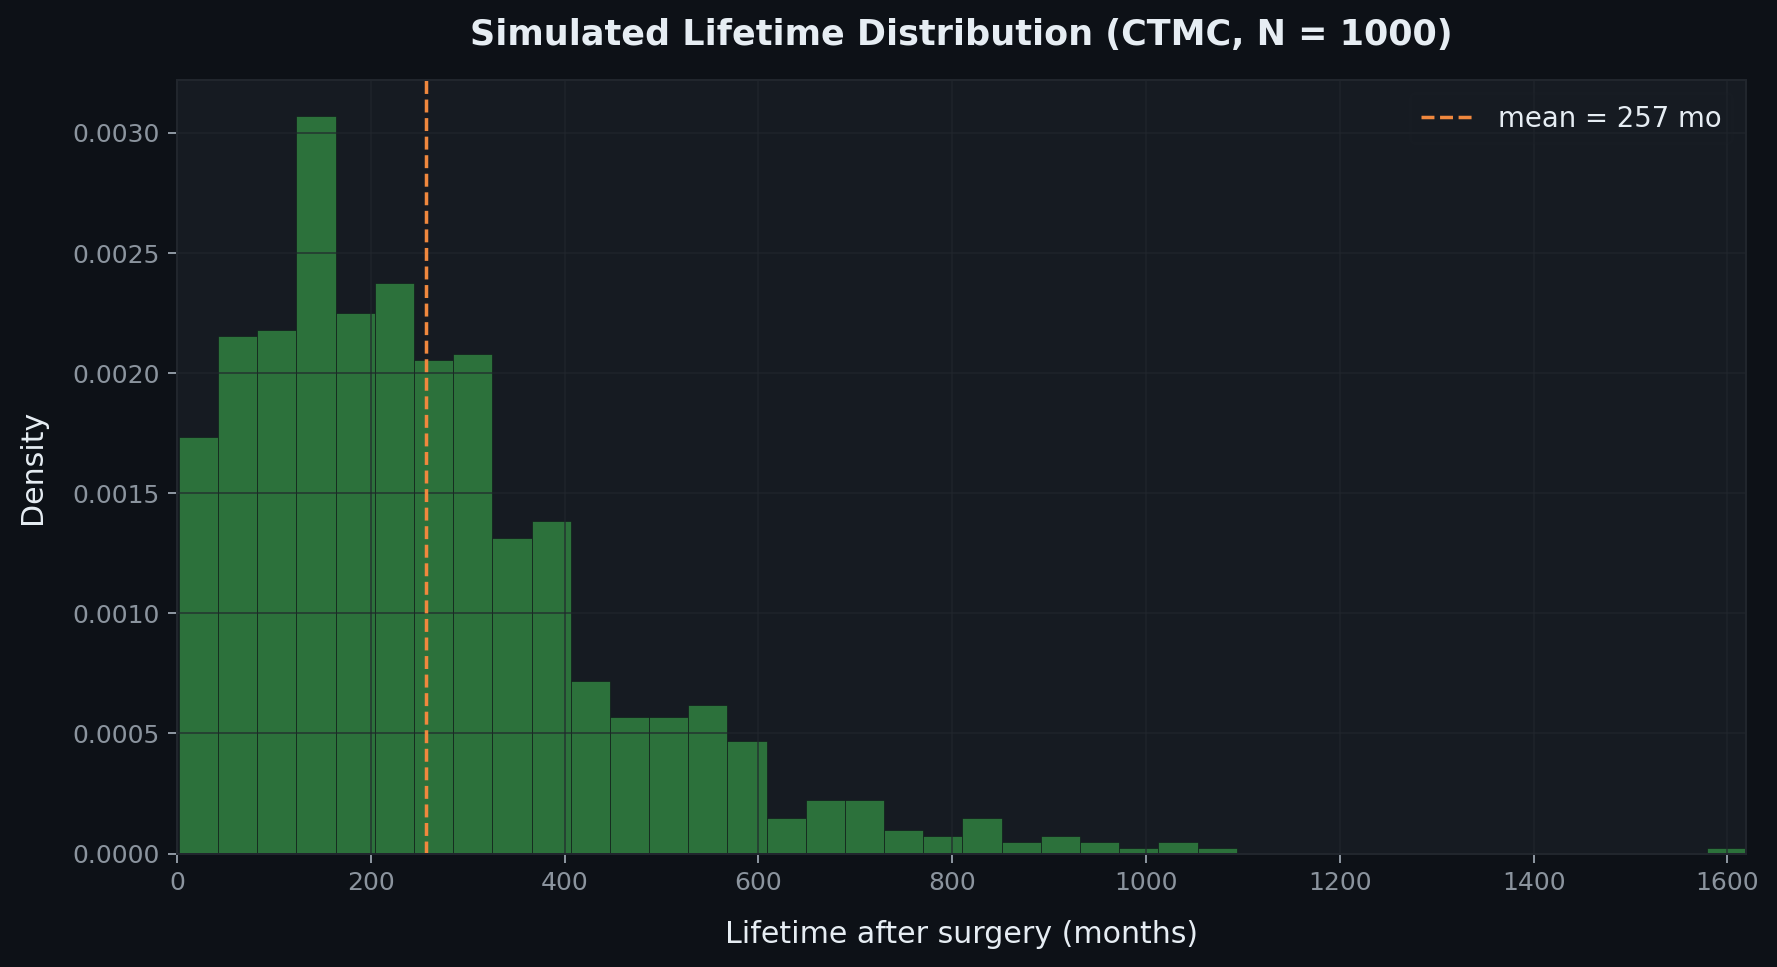
\includegraphics[width=1\linewidth]{figures/task7.png}
    \caption{Simulated lifetime distribution under the continuous-time model
    (1000 women). The dashed line marks the mean.}
    \label{fig:task7fig}
\end{figure}

The mean lifetime is $257.4$ months with a 95\% confidence interval of
$[245.7,\,269.1]$ months, computed from the normal approximation
$\bar{x}\pm 1.96\,s/\sqrt{n}$. The standard deviation is $189.0$ months. A
confidence interval for the standard deviation follows from the
$\chi^2$ distribution of the sample variance,
\[
    \left[\sqrt{\tfrac{(n-1)s^2}{\chi^2_{1-\alpha/2}}},\;
          \sqrt{\tfrac{(n-1)s^2}{\chi^2_{\alpha/2}}}\right],
\]
which gives $[181.1,\,197.7]$ months.

To find the proportion of women whose cancer has reappeared distantly after
$30.5$ months, we located the state each woman occupied at $t = 30.5$ (skipping
those who had already died) and counted the women in the distant-metastasis or
the combined local-and-distant state. This came out to $6.40\%$.

\subsection{Task 8}

Task 7 only summarises the lifetimes. Here we check whether the whole empirical
distribution matches the theory. The lifetime now follows a continuous-time
phase-type distribution with distribution function
\[
    F_T(t) = 1 - \mathbf{p}_0 \exp(\mathbf{Q}_s t)\mathbf{1},
\]
where $\mathbf{Q}_s$ is $Q$ with the death row and column removed and the matrix
exponential is evaluated with \texttt{scipy.linalg.expm}. Because the
theoretical distribution is continuous, the Kolmogorov-Smirnov test is the
natural choice rather than a binned $\chi^2$ test. We simulated 1000 women and
compared their empirical CDF against $F_T(t)$.

\begin{figure}[H]
    \centering
    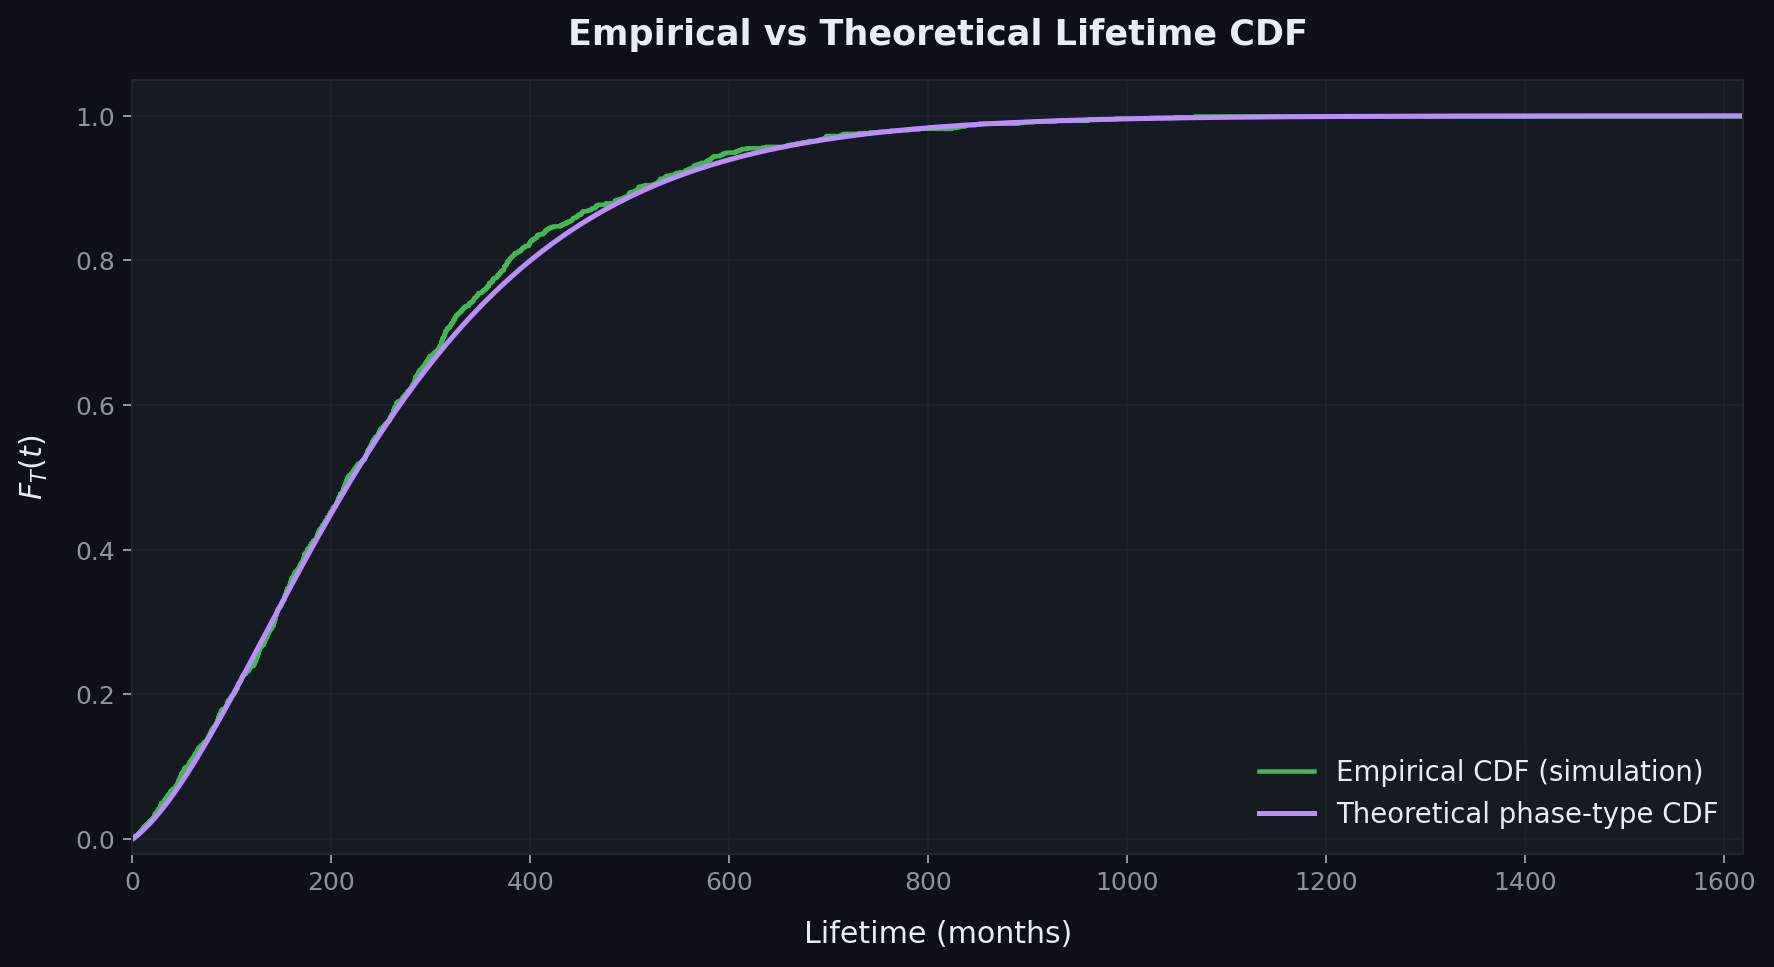
\includegraphics[width=1\linewidth]{figures/task8.png}
    \caption{Empirical CDF from 1000 simulated lifetimes against the
    theoretical phase-type CDF. The two curves sit on top of each other.}
    \label{fig:task8fig}
\end{figure}

The KS test gives a statistic of $0.0284$ with a $p$-value of $0.388$. Since
$p > 0.05$ we fail to reject the null hypothesis, so the simulated lifetimes
are consistent with the phase-type distribution. Figure~\ref{fig:task8fig}
shows the same conclusion visually: the empirical and theoretical curves are
almost indistinguishable.

\subsection{Task 9}

A preventive treatment changes the rate matrix. We filled in the diagonal
entries of the treatment matrix so that each row sums to zero, following
$q_{ii} = -\sum_{j\neq i} q_{ij}$, and simulated 1000 treated women alongside
1000 untreated women. For each group we computed the Kaplan-Meier estimate of
the survival function, $\hat{S}(t) = (N - d(t))/N$, where $d(t)$ counts the
deaths up to time $t$.

\begin{figure}[H]
    \centering
    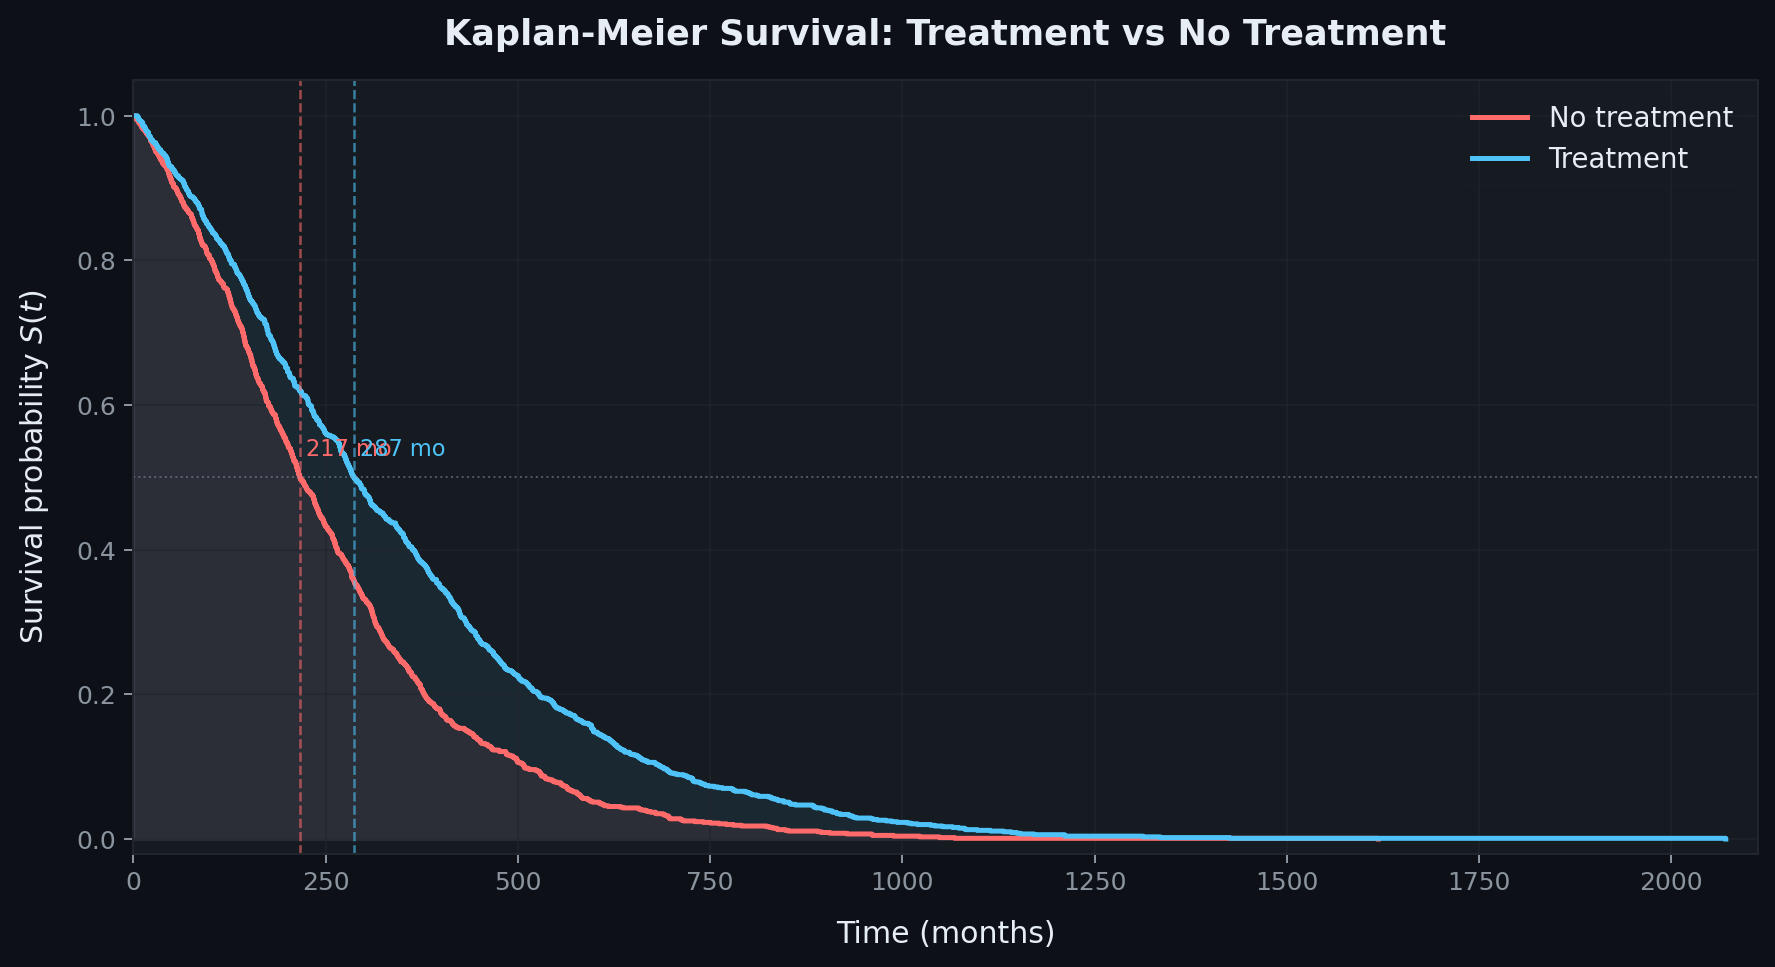
\includegraphics[width=1\linewidth]{figures/task9.png}
    \caption{Kaplan-Meier survival functions for treated and untreated women.
    Dashed lines mark the median survival of each group.}
    \label{fig:task9fig}
\end{figure}

The treatment curve lies above the no-treatment curve at every time point
(Figure~\ref{fig:task9fig}), which means treated women survive longer across
the board. The median survival rises from $216.6$ months without treatment to
$287.2$ months with it, and the mean rises from $257.4$ to $344.3$ months. The
treatment appears to have a clear positive effect on survival.

\subsection{Task 10 (Optional)}

The visual gap in Task 9 is suggestive, but we still want a formal test. The
log-rank test compares the two survival functions by looking at every death
time and asking how many deaths we would expect in each group if the two
groups really shared one survival curve. At each death time $t_i$ with $n_1$
and $n_2$ patients still at risk and $d$ total deaths, the expected deaths in
group 1 are $e_{1i} = n_1 d / (n_1 + n_2)$. The test statistic accumulates the
gap between observed and expected deaths,
\[
    Z = \frac{\left(\sum_i (d_{1i} - e_{1i})\right)^2}{\sum_i V_i},
    \qquad
    V_i = \frac{n_1 n_2\, d\, (n_1 + n_2 - d)}{(n_1 + n_2)^2 (n_1 + n_2 - 1)},
\]
and is compared against a $\chi^2$ distribution with one degree of freedom.

For our two samples the statistic is $80.14$, giving a $p$-value of
$3.49\times10^{-19}$. We reject the null hypothesis of equal survival: the
preventive treatment has a statistically significant effect.

\subsection{Task 11}

Moving from the discrete to the continuous model removes the assumption that
transitions can only happen at fixed monthly checkpoints. A patient can now
change state at any instant, which matches how disease progression actually
works. We also drop the slightly awkward feature of the discrete chain where a
patient could stay in the same state for one step with some probability; in the
continuous model the holding time is drawn directly.

What we add is the assumption that every sojourn time is exponentially
distributed, and therefore memoryless. The chance of leaving a state in the
next instant does not depend on how long the patient has already been there.
This is the same lack of duration-dependence that the discrete model had, now
expressed through the exponential holding time. For cancer this is a strong
assumption, since the risk of recurrence or death usually does change with how
long a patient has been in a given state.

The memoryless assumption can be relaxed by letting the sojourn time in a state
be Erlang distributed instead of exponential. An Erlang$(k, \lambda)$ random
variable is a sum of $k$ independent exponentials, so we can build it by
splitting one state into $k$ artificial sub-states chained in series, each with
exponential holding time $\lambda$. The patient passes through the sub-states
one after another before the real transition fires. This keeps the model a
CTMC, so the same simulation machinery still works, at the cost of a larger
state space. With enough phases an Erlang distribution can approximate a wide
range of non-exponential holding times, which makes the duration-dependence of
the real disease easier to capture.
